\documentclass[11pt]{article}
\usepackage[a4paper,margin=1in]{geometry}
\usepackage{amsmath,amssymb,amsthm}
\usepackage{graphicx}
\usepackage[hidelinks]{hyperref}

\newtheorem{theorem}{Theorem}
\newtheorem{lemma}{Lemma}
\newtheorem{remark}{Remark}

\newcommand{\N}{\mathbb N}
\newcommand{\R}{\mathbb R}
\newcommand{\cF}{\mathcal F}
\newcommand{\cS}{\mathcal S}
\newcommand{\supp}{\operatorname{supp}}
\newcommand{\depth}{\operatorname{depth}}
\newcommand{\spn}{\operatorname{span}}
\newcommand{\full}{\operatorname{full}}

\title{A Half-Parameter Partial Answer to the Fixed-Theta Tsirelson Depth Problem}
\author{Automatic math-discovery packet}
\date{June 29, 2026}

\begin{document}
\maketitle

\section*{Source Question}

The source paper is Jakub Hodor, \emph{The depth of Tsirelson's norm},
arXiv:2306.10344.  It proves that the classical case
\(T[\frac12,\cS_1]\) has depth function \(j(n)=\Theta(\sqrt n)\), and then
asks for the corresponding order when the parameter \(\theta\) varies.

\begin{figure}[h]
\centering
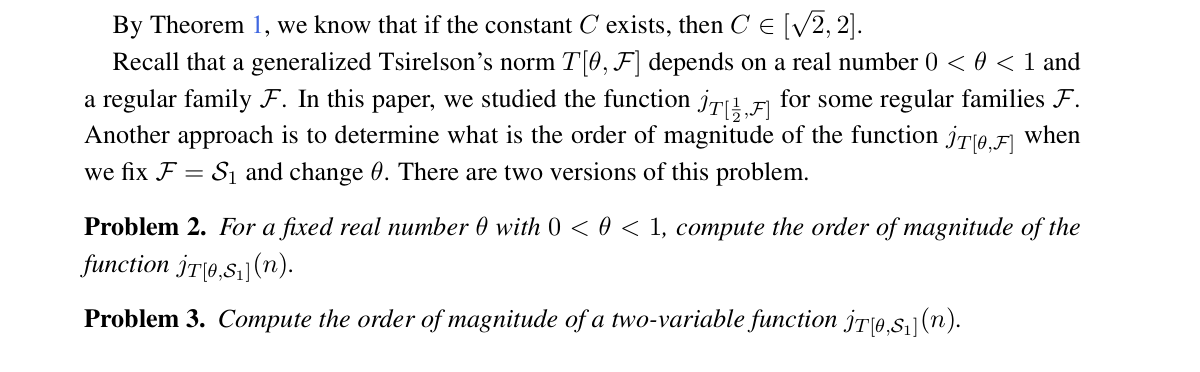
\includegraphics[width=\textwidth]{figures/open_problem_page24_crop.png}
\caption{The fixed-\(\theta\) and two-variable open problems in Hodor's paper, page 24.}
\end{figure}

\clearpage

\section*{Definitions}

Let \(0<\theta<1\) and let \(\cF\) be a regular family of finite subsets of
\(\N\).  Put
\[
  W^{\theta}_0(\cF)=\{\pm e_i^*:i\in\N\}.
\]
Given \(W^{\theta}_m(\cF)\), define \(W^{\theta}_{m+1}(\cF)\) to be
\[
  W^{\theta}_m(\cF)\cup
  \left\{\theta\sum_{i=1}^r f_i:
    f_i\in W^{\theta}_m(\cF),\
    \supp f_1<\cdots<\supp f_r,\
    \{\min\supp f_i:1\leq i\leq r\}\in\cF
  \right\}.
\]
Let \(W^\theta(\cF)=\bigcup_m W^\theta_m(\cF)\), define
\[
  \|x\|_{\theta,\cF}=\sup\{f(x):f\in W^\theta(\cF)\},
\]
and let
\[
  j_{\theta,\cF}(x)=
  \min\{\depth_\theta(f):f\in W^\theta(\cF),\ f(x)=\|x\|_{\theta,\cF}\}.
\]
Finally,
\[
  j_{\theta,\cF}(a,b)=
  \max\{j_{\theta,\cF}(x):\supp x\subset [a,b]\},\qquad
  j_{\theta,\cF}(n)=j_{\theta,\cF}(1,n).
\]
For \(\cF=\cS_1=\{E\subset\N: |E|\leq \min E\}\), this is the function
denoted \(j_{T[\theta,\cS_1]}(n)\) in the source problem.

\section*{Claim}

\begin{theorem}
For every fixed \(0<\theta\leq \frac12\),
\[
  j_{T[\theta,\cS_1]}(n)=\Theta_\theta(\sqrt n).
\]
More explicitly, the upper bound is \(j_{T[\theta,\cS_1]}(n)=O(\sqrt n)\)
with the same asymptotic constant supplied by Hodor's recursive estimate, and
the lower bound is \(j_{T[\theta,\cS_1]}(n)=\Omega_\theta(\sqrt n)\).
\end{theorem}

\section*{Proof Intuition}

Hodor's lower bound for \(\theta=\frac12\) works by placing very large
coordinates at the outside of a nested chain of full Schreier sets.  The same
forcing works for general fixed \(\theta\), provided the outer full Schreier
sets have size \(>1/\theta+1\) and the large coordinates are separated by a
factor depending on \(\theta\).

The upper bound is more delicate.  Most of Hodor's upper-bound proof is
combinatorial, but one insertion lemma uses the identity that, at
\(\theta=\frac12\), a certain norming functional is the average of two
shallower competitors.  For \(0<\theta\leq\frac12\), the same functional is a
convex combination of three competitors with weights
\((1-2\theta),\theta,\theta\).  This is exactly where the restriction
\(\theta\leq\frac12\) enters.

\section*{Lower Bound}

We use the following theta-version of the source paper's lower-bound forcing
lemma.

\begin{lemma}[Theta-forcing lower lemma]
\label{lem:theta-lower}
Let \(0<\theta<1\), let \(\cF\) be a regular family, and let \(d\in\N\).
Assume that there are \(F_1,\ldots,F_d\in\full(\cF)\) and intervals
\([a_i,b_i-1]\), \(1\leq i<d\), satisfying Hodor's nesting conditions:
\begin{enumerate}
\item \(a_i,b_i\) are consecutive in \(F_i\);
\item \(a_i\in F_{i+1}\) and \(F_{i+1}\subset [a_i,b_i-1]\);
\item for distinct \(u,v\in [a_i,b_i-1]\),
\[
  (F_i\setminus\{a_i\})\cup\{u,v\}\notin\cF.
\]
\end{enumerate}
Assume also that
\[
  |F_i|-1>\frac1\theta \qquad (1\leq i\leq d).
\]
Then there is \(x\in c_{00}^+\), supported by \(\bigcup_i F_i\), such that
\[
  j_{\theta,\cF}(x)\geq d.
\]
\end{lemma}

\begin{proof}
Choose once and for all \(L>1/(1-\theta)\).  The proof is by induction on
\(d\).  For \(d=1\), put \(x_i=1\) on \(F_1\) and \(x_i=0\) otherwise.
Since \(\theta |F_1|>1\), the functional
\(\theta\sum_{i\in F_1}e_i^*\) beats every coordinate functional, so no
depth-zero functional norms \(x\).  Hence \(j_{\theta,\cF}(x)\geq1\).

Assume the result for \(d-1\), applied to \(F_2,\ldots,F_d\).  Obtain
\(x'\geq0\), supported by \(F'=\bigcup_{i=2}^d F_i\), such that
\(j_{\theta,\cF}(x')\geq d-1\).  Let \(s=\sum_i x'_i\).  Define
\[
  x_i=\begin{cases}
    x'_i, & i\in F',\\
    Ls, & i\in F_1\setminus F',\\
    0, & \text{otherwise.}
  \end{cases}
\]
Let \(f'\) norm \(x'\), and set
\[
  g=\theta\left(f'+\sum_{i\in F_1\setminus F'}e_i^*\right).
\]
The nesting assumptions make \(g\in W^\theta(\cF)\).  Since
\(|F_1\setminus F'|=|F_1|-1\),
\[
  g(x)=\theta\|x'\|_{\theta,\cF}+
       \theta(|F_1|-1)Ls
       > Ls.
\]
Thus a norming functional \(f\) for \(x\) cannot have depth zero.

Every positive-depth functional has point coefficients at most \(\theta\).
If for some \(i_0\in F_1\setminus F'\) the coefficient \(f(e_{i_0})\) were
strictly less than \(\theta\), then, because coefficients in a norming tree are
powers of \(\theta\), we would have \(f(e_{i_0})\leq\theta^2\).  Therefore
\[
\begin{aligned}
  f(x)
  &\leq \theta\sum_{i\in (F_1\cup F')\setminus\{i_0\}}x_i
      +\theta^2 x_{i_0}  \\
  &\leq \theta(|F_1|-2)Ls+\theta s+\theta^2Ls.
\end{aligned}
\]
Because \(L>1/(1-\theta)\), the right side is strictly smaller than
\(\theta(|F_1|-1)Ls\leq g(x)\), contradicting \(f(x)=\|x\|\geq g(x)\).
Hence \(f(e_i)=\theta\) for every \(i\in F_1\setminus F'\).

It follows that
\[
  f=\theta\left(\sum_{\ell=1}^m h_\ell+
      \sum_{i\in F_1\setminus F'}e_i^*\right)
\]
for some block sequence \(h_1,\ldots,h_m\).  The third nesting condition
implies that at most one of the \(h_\ell\)'s can start inside
\([a_1,b_1-1]\).  Comparing \(f(x)\) with \(g(x)\) gives
\[
  \sum_{\ell=1}^m h_\ell(x')\geq \|x'\|_{\theta,\cF}.
\]
All summands not starting in \([a_1,b_1-1]\) vanish on \(x'\), and every
summand is bounded above by \(\|x'\|_{\theta,\cF}\).  Hence one summand
\(h_\ell\) norms \(x'\).  Since \(j_{\theta,\cF}(x')\geq d-1\), we get
\(\depth_\theta(h_\ell)\geq d-1\), and so \(\depth_\theta(f)\geq d\).
\end{proof}

Now apply the lemma to \(\cF=\cS_1\).  Let
\[
  q_\theta=\left\lfloor\frac1\theta\right\rfloor+2.
\]
For a given \(d\), define integers \(B_{d+1}=q_\theta+d+1\) and
\[
  B_i=B_{i+1}+q_\theta+i-3 \qquad (1\leq i\leq d).
\]
Set
\[
  F_i=\{q_\theta+i-1,q_\theta+i\}\cup [B_{i+1},B_i-1].
\]
Then \(F_i\) is a full Schreier set: its cardinality is
\(q_\theta+i-1=\min F_i\).  The sets satisfy the nesting hypotheses above,
and \(|F_i|-1>1/\theta\).  Therefore
\[
  j_{\theta,\cS_1}(N_d)\geq d,
\]
where
\[
  N_d=\max F_1
      =q_\theta+d(q_\theta-2)+\frac{d(d+1)}2.
\]
This proves \(j_{\theta,\cS_1}(n)=\Omega_\theta(\sqrt n)\).

\section*{Upper Bound for \(0<\theta\leq 1/2\)}

We recall only the coefficient-sensitive part of Hodor's upper-bound proof and
explain its theta-version.  The remaining steps use the same full-set and
Schreier-family combinatorics as in the source paper.

The easy replacement lemmas remain valid with \(\frac12\) replaced by
\(\theta\): if a positive-depth functional \(f\) has support in \(\cF\), then
\(\theta\sum_{i\in\supp f}e_i^*\) is not worse than \(f\) on positive vectors;
and a norming functional can be replaced by one that is either shallow or
\(\cF\)-full.

The insertion lemma is the only place where the value \(\frac12\) is special.
Suppose \(\cF\) has the insertion property, \(g'\) is a norming full
functional chosen with maximal possible minimum support, and
\[
  g'=\theta(g_1+\cdots+g_r), \qquad
  g_1=\theta(t_1+\cdots+t_s),
\]
with \(t_1\) still too deep.  Hodor forms two inserted competitors and uses an
average identity.  For \(0<\theta\leq\frac12\), define
\[
\begin{aligned}
  u_0&=\theta(g_2+\cdots+g_r),\\
  u_1&=\theta(t_1+g_2+\cdots+g_r),\\
  u_2&=\theta(t_2+\cdots+t_s+g_2+\cdots+g_r).
\end{aligned}
\]
Empty sums are simply omitted; the degenerate one-branch cases are easier,
because a useless scalar branch can be replaced by its child.  The insertion
property and heredity of \(\cF\) make these functionals admissible.  A direct
coefficient check gives
\[
  g'=(1-2\theta)u_0+\theta u_1+\theta u_2.
\]
Since \(g'\) norms \(x\), and each \(u_i(x)\leq \|x\|_{\theta,\cF}\), every
competitor with positive coefficient in this convex combination also norms
\(x\).  In particular, \(u_2\) norms \(x\), has no larger depth than \(g'\),
and has strictly larger minimum support.  Applying the shallow-or-full
replacement lemma to \(u_2\) contradicts the choice of \(g'\).  Thus Hodor's
strengthened insertion lemma remains true for \(0<\theta\leq\frac12\).

Consequently the realizing-sequence lemma and the recursive estimate for
\(\cS_\varphi\) hold verbatim in this parameter range.  For
\(\varphi(a)=a\), i.e. \(\cS_\varphi=\cS_1\), one obtains:
if \(a\leq b\) and \(|[a,b]|\leq a\), then
\[
  j_{\theta,\cS_1}(a,b)\leq 1,
\]
and otherwise
\[
  j_{\theta,\cS_1}(a,b)\leq
  2+\max\{j_{\theta,\cS_1}(a+i,b-a+i+1):1\leq i<a\}.
\]
The same induction as in Hodor's Section 7.1 yields
\[
  n\leq \sum_{i=1}^{c+1}i-c
  \quad\Longrightarrow\quad
  j_{\theta,\cS_1}(n)\leq 2c+1.
\]
Choosing \(c=O(\sqrt n)\) proves
\[
  j_{\theta,\cS_1}(n)=O(\sqrt n)
\]
for every \(0<\theta\leq\frac12\).

Combining this with the lower bound completes the proof of the theorem.

\section*{Why This Is Only Partial}

The modified insertion step uses a convex combination with coefficient
\(1-2\theta\).  When \(\theta>\frac12\), this coefficient is negative, and the
argument no longer proves that a later-support competitor also norms the
vector.  A tempting alternative is to use linear-depth chain functionals on
supports of size \(O(d)\), but finite-dimensional LP checks for small supports
show that these chains do not uniformly beat all shallower functionals except
in very small or very large-\(\theta\) toy cases.  No proof-grade replacement
for the insertion lemma in the range \(\theta>\frac12\) is included here.

\section*{Literature and Novelty Check}

Before promotion, the cheap run indexes were searched for arXiv \texttt{2306.10344},
for \texttt{depth of Tsirelson}, and for the exact theta-Schreier keywords; no prior
run packet for this target was found.  A bounded web search on June 29, 2026
used the phrases:
\begin{itemize}
\item \texttt{j\_\{T[theta,S\_1]\}},
\item \texttt{T[theta,S\_1] j Tsirelson depth},
\item \texttt{The depth of Tsirelson's norm theta Schreier}.
\end{itemize}
The search found the source paper and no later exact answer to the
\(\theta\leq\frac12\) subcase.  Novelty confidence is therefore bounded rather
than absolute.

\section*{Verification Notes}

The proof is not computational.  The included script
\texttt{code/theta\_chain\_lp\_probe.py} records only a finite LP diagnostic for
the unpromoted \(\theta>\frac12\) chain idea.  The main human-review focus
should be the two analytic modifications: Lemma~\ref{lem:theta-lower} and the
convex-combination replacement in the insertion lemma.

\begin{thebibliography}{9}

\bibitem{Hodor}
J. Hodor,
\emph{The depth of Tsirelson's norm},
arXiv:2306.10344, 2023.

\end{thebibliography}

\end{document}
